\section{Architecture logicielle}

	Plutôt qu'implémenter les nouvelles fonctionnalités présentées dans les parties suivantes directement dans ADTool, nous avons fait le choix de créer un nouveau logiciel nommé \glasir{} qui utilisera cet éditeur d'arbres. Deux raisons nous ont poussés à prendre cette décision. 
La première est de séparer l'analyse et l'édition des ADTrees, afin d'avoir des logiciels dédiés à leur tâche. Cette solution nous permet d'utiliser des technologies différentes de celles d'ADTool, enrichissant ainsi notre formation. \glasir{} se chargera de la partie \textit{analyse}, et ADTool de la partie \textit{édition des arbres} sous forme de sous-fenêtre de \glasir{}. On peut voir sur la {\sc Figure} \ref{fig:architecture_Glasir} l'intégration d'ADTool dans l'architecture de \glasir. 

	\begin{figure}[h!]
		\centering
			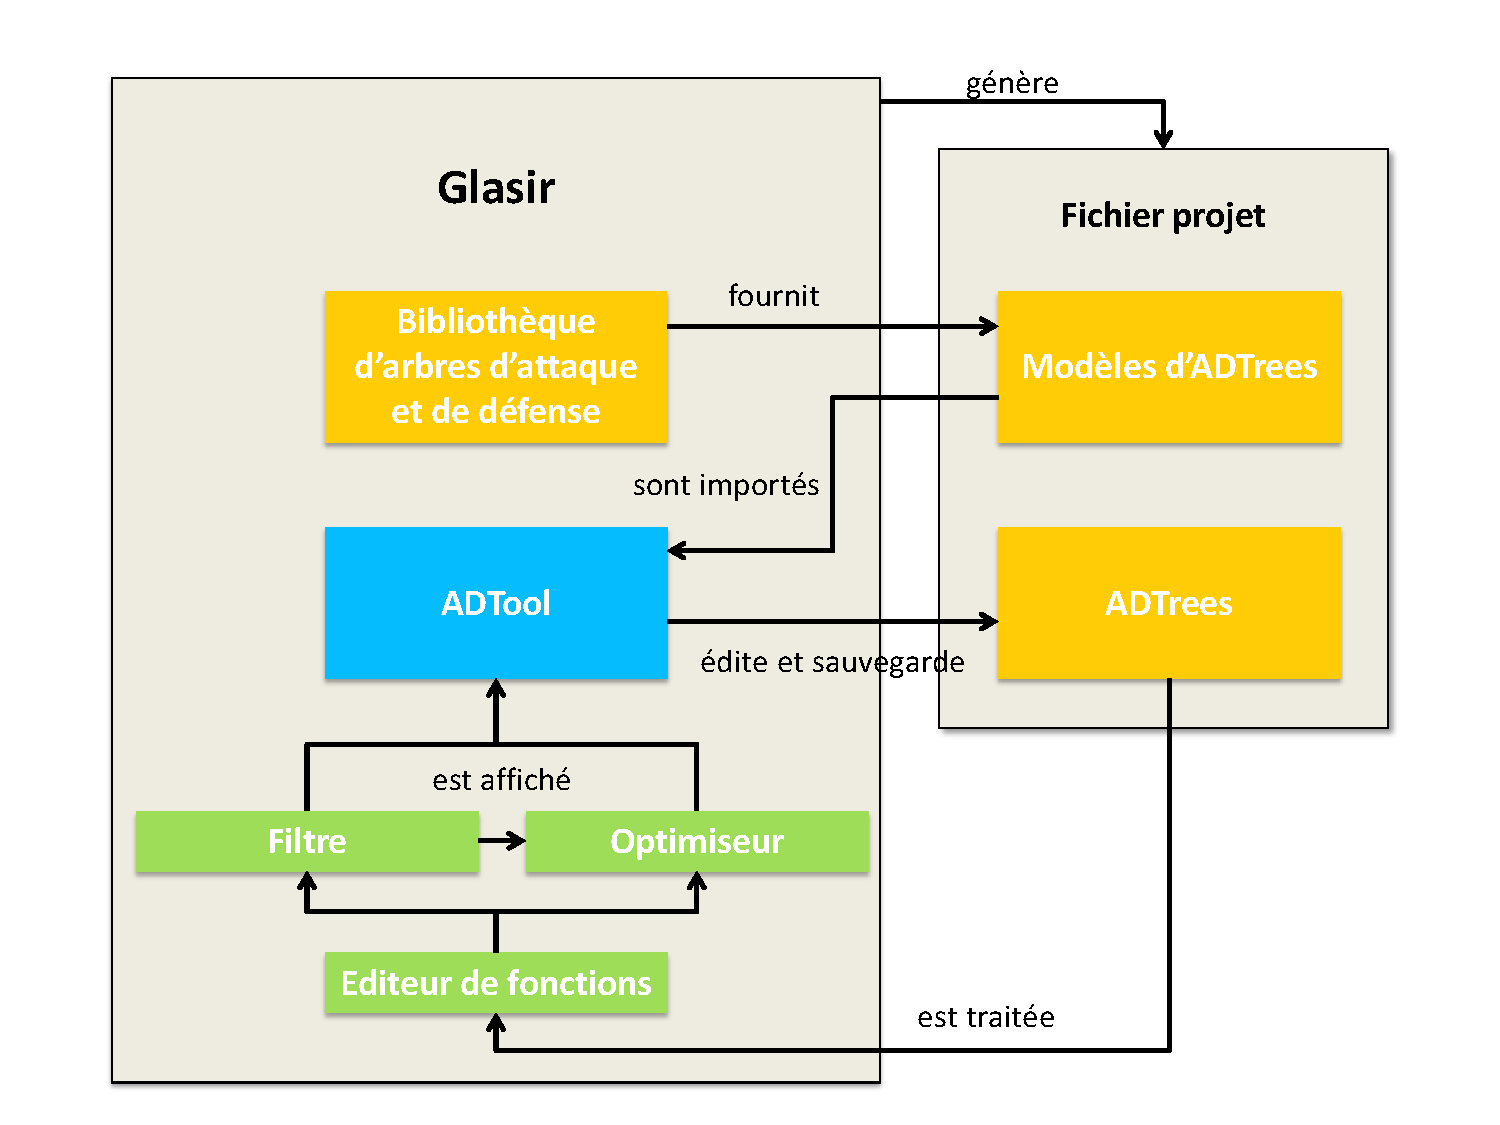
\includegraphics[width=0.8\textwidth]{figure/archiGlasir.pdf}
		\caption{Architecture du logiciel \glasir.}
		\label{fig:architecture_Glasir}
	\end{figure}

	Tel qu'illustré sur la {\sc Figure} \ref{fig:architecture_Glasir}, \glasir{} est constitué d'une bibliothèque d'ADTrees, d'ADTool et des nouvelles fonctionnalités d'analyse. L'utilisation de \glasir{} se fait au travers de fichiers projets, qui contiennent les ADTrees du projet en cours ainsi que les modèles génériques d'ADTrees, provenant de la bibliothèque d'ADTrees de \glasir{}, qui sont utilisés dans le cadre du projet.
	
	Lors d'un projet quelconque, Glasir commence par créer le fichier projet correspondant. L'expert va alors créer ou importer ses ADTrees grâce à ADTool. Les éventuels modèles de la bibliothèque d'ADTrees utilisés dans le cadre du projet seront également sauvegardés dans le fichier projet, pour gérer leurs éventuels modifications sans impacter la bibliothèque d'arbres de \glasir{}. L'expert pourra alors définir ses paramètres de synthèse avec l'éditeur de fonction, et filtrer ou chercher le chemin optimal grâce au Filtre et à l'optimiseur. L'arbre élagé par ces modules sera alors affiché par ADTool.